\section{超弾性(Hyperelasticity)}
\subsection{超弾性とは}
\begin{itemize}
	\item 物体を構成する物質の力学的特性の数理的表現のひとつ
	\item ひずみエネルギー密度関数(単位体積あたりのひずみエネルギーを表す弾性ポテンシャル)を有することが特徴
	\item 超弾性を有する物質を超弾性体とよび、ゴムの最も簡易なモデルとして登場したことに由来して、数10 %~数100%の大ひずみ状態を想定
\end{itemize}
\vspace{-\baselineskip}
\begin{flushright}
	\href{https://ja.wikipedia.org/wiki/%E8%B6%85%E5%BC%BE%E6%80%A7}{Wikipedia「超弾性」より}
\end{flushright}
\vspace{-\baselineskip}
\subsection{ゴム材料(エラストマ)の単軸引張試験結果}
\vspace{-\baselineskip}
\begin{figure}[H]
	\caption{単軸引張試験の例}
	\label{fig:002}
	\centering
	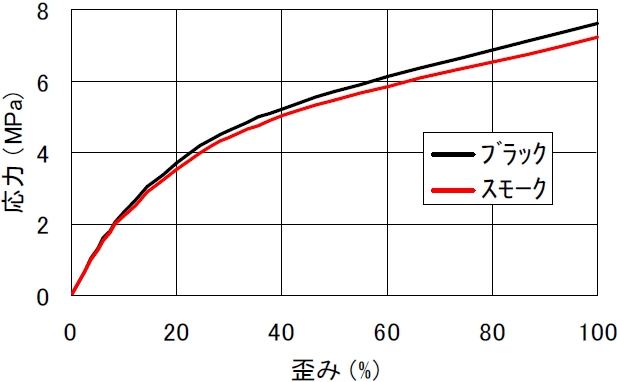
\includegraphics[width=0.4\columnwidth]{fig/tensile test.png}
\end{figure}
\section{Code\_Asterの超弾性材料}
\subsection{Code\_Asterで採用されている超弾性材料}
\begin{itemize}
	\item Signorini(シニョリーニ)
	\item Mooney-Rivlin(ムーニー・リブリン)
	\item Néo-Hookéen(ネオ・ファッキアン)
\end{itemize}
\begin{itemize}
	\item 商用ソフトにあるような以下の材料モデルには未対応
	      \begin{itemize}
		      \item Polynominal(多項式)
		      \item Yeoh(ヨー)
		      \item Ogden(オクデン)
		      \item Arruda-Boyce(アルーダ・ボイス)
		      \item Gent(ジェント)
		      \item Blatz-Ko(ブラッツ・コウ)
	      \end{itemize}
\end{itemize}
\clearpage
\subsection{キーワード因子ELAS\_HYPER}
材料を特徴づけるパラメータは、\textit{DEFI\_MATERIAU}で\textit{ELAS\_HYPER}というキーワードで定義されています。
\vspace{\baselineskip}
大きな変位、回転、および変形 (\textit{DEFORMATION=' GROT\_GDEP'}) をサポートしています。\footnote{この挙動では、熱による変形を考慮することはできません。}
\begin{itemize}
	\item 対応要素:\textit{3D}(3次元)、\textit{D\_PLAN}(平面ひずみ)、\textit{C\_PLAN}(平面応力)
	\item Example:テストケース\textit{SSNV187}
	\item Reference material \textit{R5.03.19}
\end{itemize}
\clearpage
\subsection{ELAS\_HYPER構文}
\begin{lstlisting}[caption =Syntax, label = Syntax]
| ELAS_HYPER= _F (
               ♦   C10   =   c10,     [R]
               ◇   C01   =   / c01,   [R]
                             / 0.0,    [DEFECT]
               ◇   C20   =   / c20,   [R]
                             / 0.0,    [DEFECT]
               ◇   RHO   =   / rho,   [R]
                             / 0.0,    [DEFECT]
               ◇   NAKED =   naked,   [R]
               ◇   K     =   K        [R]
               )
\end{lstlisting}
\clearpage
\subsubsection{オペランド\textit{C01}、\textit{C10}、\textit{C20}}
\textit{C01 = c01} 、\textit{ C10 = c10}、 \textit{C20 = c20}
超弾性多項式の3つのポテンシャル関数。\\
単位は$N/mm^{2}$
\begin{itemize}
	\item \textit{C20}のみがNullの場合、Mooney-Rivlin(ムーニー・リブリン)型の材料モデル。
	\item \textit{C01}と\textit{C20}がNullの場合、Néo-Hookéen(ネオ・ファッキアン)型の材料モデル。
\end{itemize}
\textit{6(C01+C10)=E}のように\textit{C10}と\textit{C01}を取る場合、小さな変形では弾性非圧縮性を持つ材料となります。
ここで、\textit{E}はヤング率です。
\vspace{\baselineskip}
\begin{table}[H]
	\centering
	\begin{tabular}{@{}cccc@{}}
		\toprule
		              & \textit{C01} & \textit{C10} & \textit{C20} \\ \midrule
		Signorini     & YES          & YES          & YES          \\
		Mooney-Rivlin & YES          & YES          & Null         \\
		Néo-Hookéen   & Null         & YES          & Null         \\ \bottomrule
	\end{tabular}
\end{table}
\clearpage
\subsubsection{オペランド\textit{NAKED}と\textit{K}}
\textit{NAKED = naked}\\
ポアソン比。
-1<$\nu$<0.5であることを確認します。
\textit{K = K}\\
体積弾性率。
これらの2つのパラメータは1つだけを用い、もう1つを除外します。\\
これらのパラメータは、材料の圧縮性をほぼ定量化します。\\
ユーザが提供する体積弾性率\textit{K}が存在すれば、それを使用します。\\
存在しない場合は、次式(\ref{compressibility})を用いて計算します。
\begin{equation}
	\label{compressibility}
	K=\frac{6(C01+C10)}{3(1-2\nu)}
\end{equation}
$\nu$は0.5に近い値を取ることができますが,厳密には決して等しくはありません。\\
$\nu$が0.5に近すぎる場合、ポアソン比またはその体積弾性率をチェックするように、エラーメッセージが表示されます。\\
体積弾性率が大きいほど、材料は非圧縮性が高くなります。
\subsubsection{オペランド\textit{RHO}}
\textit{RHO = rho}\\
質量密度(関数型の概念を受けつけません)。
サイズについてのチェックはありません。